\documentclass[compress,red]{beamer}
\usepackage[utf8]{inputenc}
\usepackage{ucs}
\usepackage{amsmath}
\usepackage{amsfonts}
\usepackage{amssymb}
\usepackage[russian]{babel}
\usepackage{graphicx}
\usepackage{wrapfig}
\usepackage[normalem]{ulem}

\usepackage{tikz}
\usepackage{verbatim}

\usepackage{color}
\usepackage{xcolor}
\usepackage{listings}

\usepackage{caption}
\DeclareCaptionFont{white}{\color{white}}
\DeclareCaptionFormat{listing}{\colorbox{gray}{\parbox{\textwidth}{#1#2#3}}}
\captionsetup[lstlisting]{format=listing,labelfont=white,textfont=white}

\usetikzlibrary{calc,trees,positioning,arrows,chains,shapes.geometric,%
    decorations.pathreplacing,decorations.pathmorphing,shapes,%
    matrix,shapes.symbols}

\tikzset{
>=stealth',
  punktchain/.style={
    rectangle, 
    rounded corners, 
    % fill=black!10,
    draw=black, very thick,
    text width=10em, 
    minimum height=3em, 
    text centered, 
    on chain},
  line/.style={draw, thick, <-},
  element/.style={
    tape,
    top color=white,
    bottom color=blue!50!black!60!,
    minimum width=8em,
    draw=blue!40!black!90, very thick,
    text width=10em, 
    minimum height=1.5em, 
    text centered, 
    on chain},
  every join/.style={->, thick,shorten <=1pt},
  decoration={brace},
  tuborg/.style={decorate},
  tubnode/.style={midway, right=2pt},
}

\mode<presentation>

\usetheme{Warsaw}

\definecolor{Red}{rgb}{1,0,0}
\definecolor{Blue}{rgb}{0,0,1}
\definecolor{Green}{rgb}{0,1,0}
\definecolor{magenta}{rgb}{1,0,.6}
\definecolor{lightblue}{rgb}{0,.5,1}
\definecolor{lightpurple}{rgb}{.6,.4,1}
\definecolor{gold}{rgb}{.6,.5,0}
\definecolor{orange}{rgb}{1,0.4,0}
\definecolor{hotpink}{rgb}{1,0,0.5}
\definecolor{newcolor2}{rgb}{.5,.3,.5}
\definecolor{newcolor}{rgb}{0,.3,1}
\definecolor{newcolor3}{rgb}{1,0,.35}
\definecolor{darkgreen1}{rgb}{0, .35, 0}
\definecolor{darkgreen}{rgb}{0, .6, 0}
\definecolor{darkred}{rgb}{.75,0,0}

\xdefinecolor{olive}{cmyk}{0.64,0,0.95,0.4}
\xdefinecolor{purpleish}{cmyk}{0.75,0.75,0,0}

\useoutertheme[subsection=false]{smoothbars}


\title{Инкапсуляция и полиформизм}
\author{Информатика \\ 10-11 классы}

%\usecolortheme{dolphin}


\begin{document}
%%титульная страница
\maketitle
%% основные моменты

\section{Разбор задач}

\subsection{Разбор задач}
\begin{frame}
  \frametitle{Разбор задач.}
  \begin{itemize}
    \item \textbf{Задача 1}. Написать класс Прямоугольник --- наследник Polygon. Определить в нём метод подсчёта площади. Проверить корректность его работы.
    \item Самым простым способом подсчёта площади является перемножение длинной стороны прямоугольника на короткую. Данные о сторонах мы имеем в свойстве sides, поэтому задача становится весьма несложной.
  \end{itemize}
\end{frame}

\subsection{Задача 1}
\begin{frame}[fragile]
  \frametitle{Задача 1}
  \scriptsize{
  \begin{lstlisting}[language=ruby,basicstyle=\footnotesize,label=ruby1,caption=Задача 1]
    class Polygon
      ...
    end
    
    class Rectangle < Polygon
      def square
        @square = @sides[0]*@sides[1]
      end
    end
    
    r = Rectangle.new
    r.sides = [10,2,10,2]
    puts r.square
  \end{lstlisting}
  }
  
\end{frame}

\subsection{Задача 2}
\begin{frame}[fragile]
  \frametitle{Задача 2}
  \begin{itemize}
    \item \textbf{Задача 2.} Написать в классе Прямоугольник метод, определяющий, является ли прямоугольник квадратом. Метод должен возвращать булевский ответ. Проверить корректность работы метода.
    \item Вспомним, что булевский ответ --- это истина или ложь. В качестве правил хорошего тона булевские методы следует оканчивать на знак вопроса. 
    \item Назовём наш метод square?.
    \item \textbf{Алгоритм:} прямоугольник является квадратом, когда все его углы и стороны равны между собой. Достаточно проверить три угла, так как чётвёртый получается вычитанием из 360.
  \end{itemize}
\end{frame}

\subsection{Разбор задачи 2}
\begin{frame}[fragile]
  \frametitle{Решение задачи 2}
    \scriptsize{
    \begin{lstlisting}[language=ruby,basicstyle=\footnotesize,label=ruby2,caption=Задача 2]
      class Rectangle < Polygon
        ...
        def square?
          if ( (@sides[0] == @sides[1]) &&
               (@sides[1] == @sides[2]) &&
               (@sides[2] == @sides[3]) &&
               (@corners[0] == 90) &&
               (@corners[1] == 90) &&
               (@corners[2] == 90) 
               )
            true
          else
            false
          end
        end
      end
    \end{lstlisting}
    }
\end{frame}

\subsection{Задача 3}
\begin{frame}[fragile]
  \frametitle{Задача 3}
  \begin{itemize}
    \item \textbf{Задача 3}. Создать в классе Треугольник метод, проверяющий, является ли данный треугольник прямоугольным. Проверить корректность работы метода.
    \item \textbf{Алгоритм:} треугольник является прямоугольным, если выполнено условие теоремы Пифагора: сумма квадратов катетов равна квадрату гипотенузы.
    \item Для быстрого определения, какая сторона самая большая, используем метод sort для массива сторон.
  \end{itemize}
\end{frame}

\subsection{Разбор задачи 3}
\begin{frame}[fragile]
  \frametitle{Решение задачи 3}
  \scriptsize{
  \begin{lstlisting}[language=ruby,basicstyle=\footnotesize,label=ruby3,caption=Задача 3]
    class Triangle < Polygon
      ...
      def rectangular?
        sides = @sides.sort
        if (sides[2]**2 == (sides[0]**2 + sides[1]**2))
          true
        else
          false
        end
      end
      ...
    end
  \end{lstlisting}
  }
  
\end{frame}

\section{Инкапсуляция}
\begin{frame}
  \begin{center}
    \Huge{Три кита ООП}
    \centerline{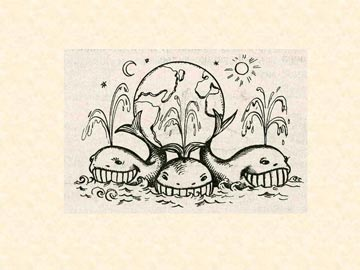
\includegraphics[width=0.6\textwidth]{images/3whales.jpg}}
  \end{center}
\end{frame}

\subsection{Три кита ООП}
\begin{frame}
  \begin{center}
    \begin{itemize}
      \item \Huge{Инкапсуляция}
      \item \Huge{Наследование}
      \item \Huge{Полиморфизм}
    \end{itemize}
  \end{center}
\end{frame}

\subsection{Три кита ООП 2}
\begin{frame}
  \begin{center}
    \begin{itemize}
      \item \Huge{Инкапсуляция}
      \item \Huge{\sout{Наследование}}
      \item \Huge{Полиморфизм}
    \end{itemize}
  \end{center}
\end{frame}

\subsection{Инкапсуляция}
\begin{frame}
  \begin{center}
    \Huge{Инкапсуляция}
  \end{center}
\end{frame}

\subsection{Инкапсуляция 2}
\begin{frame}[fragile]
  \frametitle{Инкапсуляция}
  \begin{itemize}
    \item Объектно--ориентированное программирование позволяет использовать парадигму чёрного ящика для сокрытия логики приложения.
    \item Написав однажды какой-либо метод, нет смысла впоследствии вникать в его содержимое.
    \item Более того, другие программисты могут вообще не знать реализацию конкретного метода, но вполне уметь его использовать.
    \item Такой подход в объектно-ориентированном программировании называется \emph{инкапсуляция}.
  \end{itemize}
\end{frame}


\subsection{Инкапсуляция пример}
\begin{frame}[fragile]
  \frametitle{Пример с уравнением ax + b = c}
  \scriptsize{
  \begin{lstlisting}[language=ruby,basicstyle=\footnotesize,label=ruby4,caption=Инкапсуляция]
    class LinearEquation
      attr_accessor :a, :b, :c
      def initialize(a,b,c)
        @a = a
        @b = b
        @c = c
      end
      def solve
        if (@a == 0)
          return "any" if (@b == @c)
          return "no solutions"
        else
          x = (@c - @b) / @a
        end
      end
    end
  \end{lstlisting}
  }
\end{frame}

\subsection{Разбор примера}
\begin{frame}[fragile]
  \frametitle{Разбор кода}
  \begin{itemize}
    \item В этом коде были использованы несколько новых конструкций. Вы можете его не понимать. Но самое важное --- он работает, а, значит, в соответствии с принципом инкапсуляции (в данном случае --- сокрытия) вы можете его использовать.
    \item Например, решим уравнение: 2x - 4 = 6.
  \end{itemize}
  \scriptsize{
  \begin{lstlisting}[language=ruby,basicstyle=\footnotesize,label=ruby5,caption=Используем код]
    eq = LinearEquation.new(2, -4, 6)
    puts eq.solve
  \end{lstlisting}
  \begin{itemize}
    \item Итого: инкапсуляция позволяет использовать любой код без необходимости понимать, как оно устроено внутри.
  \end{itemize}
  }
\end{frame}

\subsection{Конструкторы}
\begin{frame}[fragile]
  \frametitle{Конструкторы}
  \begin{itemize}
    \item В классе LinearEquation мы использовали неизвестный нам ранее метод \textbf{initialize}. 
    \item Это --- специальный метод. Он называется \textbf{конструктор}.
    \item Конструктор --- это метод, который вызывается \textbf{при создании} нового объекта.
    \item Конструкторы используются для автоматизации задач, которые нужно выполнить при создании объекта.
    \item В нашем примере мы сразу в конструктор передаём исходные данные задачи, чтобы не ``забивать'' их вручную.
    \item Для передачи данных в конструктор мы в метод \textbf{new} передаём нужные параметры.
  \end{itemize}
\end{frame}

\subsection{Дополнительно}
\begin{frame}[fragile]
  \frametitle{Дополнительно об инкапсуляции}
  \begin{itemize}
    \item Помимо уже рассмотреного, одной из возможностей инкапсуляции является сокрытие методов.
    \item Не вдаваясь сейчас в подробности, укажем, что существуют три возможных \emph{видимости} методов:
      \begin{enumerate}
        \item Публичный метод
        \item Приватный метод
        \item Защищённый метод
      \end{enumerate}
    \item Идея инкапсуляции заключается в сокрытии с помощью видимости тех методов, к которым нежелательно давать доступ программисту. Это позволяет уменьшить количество ошибок в программе.
  \end{itemize}
\end{frame}

\section{Полиморфизм}

\subsection{Полиморфизм заголовок}
\begin{frame}
  \begin{center}
    \Huge{Полиморфизм}
  \end{center}
\end{frame}

\subsection{Полиморфизм}
\begin{frame}[fragile]
  \frametitle{Полиморфизм}
  \begin{itemize}
    \item Рассмотрим класс \textbf{Человек}. У класса Человек есть свойства \emph{фамилия, имя, отчество} и метод \textbf{обратиться по имени}.
    \item К большинству людей в России принято обращаться по имени--отчеству.
    \item Однако к школьникам, обычно, обращаются по имени.
    \item Итого, один и тот же метод для разных классов имеет разные реализации.
    \item Возможность похожих классов (например, наследников) иметь различную реализацию одного и того же метода называется \textbf{полиморфизмом}.
  \end{itemize}
\end{frame}

\subsection{Пример полиморфизма}
\begin{frame}[fragile]
  \frametitle{Пример полиморфизма}
  \scriptsize{
  \begin{lstlisting}[language=ruby,basicstyle=\footnotesize,label=ruby6,caption=Полиморфизм]
    class Person
      attr_accessor :first_name, :last_name, :middle_name, :job
      def getName
        @first_name + ' ' + @middle_name
      end
    end
    
    class Teacher < Person
    end
    
    class Student < Person
      def getName
        @first_name
      end
    end
  \end{lstlisting}
  }
  
\end{frame}

\subsection{Polizei}
\begin{frame}[fragile]
  \frametitle{Polizei}
  \centerline{
\includegraphics[width=0.6\textwidth]{images/herr_polizei.jpg}}
\end{frame}

\subsection{Пример полиморфизма 2}
\begin{frame}[fragile]
  \frametitle{Пример полиморфизма}
  \scriptsize{
  \begin{lstlisting}[language=ruby,basicstyle=\footnotesize,label=ruby7,caption=Полиморфизм]
    class Polizei < Person # really Person???
      def getName
        'Herr Polizei'
      end
    end
    
    p = Polizei.new
    puts p.getName
    
  \end{lstlisting}
  }
  
\end{frame}

\subsection{Использование полиморфизма}
\begin{frame}[fragile]
  \frametitle{Для чего нужен полиморфизм?}
  \begin{itemize}
    \item С помощью полиморфизма можно переопределять методы родительского класса.
    \item Часто имеется следующая ситуация: в 90\% случаев методы наследников полностью идентичны. В этом случае общий метод выносят в класс--родитель, чтобы не дублировать код.
    \item Однако в 10\% случаев есть необходимость по-другому реализовать метод.
    \item Чтобы не вставлять в метод проверки и условия, используют полиморфизм, переопределяя метод только там, где нужно.
    \item \textbf{Самостоятельное изучение}. Перегрузка методов, перегрузка / переопределение операций.
  \end{itemize}
\end{frame}

\subsection{Полиморфизм и конструкторы}
\begin{frame}[fragile]
  \frametitle{Конструкторы при полиморфизме}
  \begin{itemize}
    \item В созданном классе <<Учитель>> мы можем автоматически проставлять свойство job. 
    \item Это проще всего сделать с помощью конструктора.
  \end{itemize}
  \scriptsize{
  \begin{lstlisting}[language=ruby,basicstyle=\footnotesize,label=ruby8,caption=Конструктор в полиморфизме]
    class Teacher < Person
      def initialize
        @job = "Teacher"
      end
    end
    
    t = Teacher.new
    puts t.job
  \end{lstlisting}
  }
  
\end{frame}

\subsection{Конструктор родителя}
\begin{frame}[fragile]
  \frametitle{Конструктор родителя}
  \begin{itemize}
    \item А что делать, если мы хотим вызвать и конструктор родителя, и текущий? Ведь если мы переопределяем с помощью полиморфизма метод initialize, то ``старый'' забывается.
    \item Для этого в ruby есть специальный метод \textbf{super}.
    \item Простой вызов этого метода вызовет конструктор родителя.
    \item Разумеется, в метод super можно передавать аргументы.
    \item В предложенном на следующем слайде примере код выведет на экран две строчки: <<B>>, <<A>>.
  \end{itemize}
  
\end{frame}

\subsection{Конструктор родителя код}
\begin{frame}[fragile]
  \frametitle{Код конструктора родителя}
  \scriptsize{
  \begin{lstlisting}[language=ruby,basicstyle=\footnotesize,label=ruby9,caption=Конструктор родителя]
    class A
      def initialize(label)
        puts label
      end
    end
    
    class B < A
      def initialize
        puts "B"
        super("A")
      end
    end
    
    b = B.new
  \end{lstlisting}
  }
\end{frame}

\section{Задание}
\subsection{Задание}
\begin{frame}[fragile]
  \frametitle{Задание}
  \begin{itemize}
    \item Создать следующие классы: человек, ученик, ученик--раздолбай, учитель, директор. 
    \item Каждый человек имеет: фамилию, имя, отчество, год рождения. Наследование определено в соответствии со здравым смыслом (ученик--раздолбай --- наследник ученика). Все сущности имеют методы:
     \begin{enumerate}
      \item Посчитать возраст (getAges).
      \item обратиться по имени (getName) по правилу: учитель и директор --- имя + отчество, ученик --- имя, ученик-раздолбай --- ``Бяка'' + имя. 
      \item булевский метод главный (head?): для директора возвращается истина, для остальных --- ложь.
     \end{enumerate} 
    \item ФИО и год рождения должно задаваться в конструкторе.
    \item После реализации создать экземпляры каждого класса и вызвать для них методы getName, getAges, head?.
  \end{itemize}
\end{frame}

\subsection{Сложное задание}
\begin{frame}[fragile]
  \frametitle{Сложное задание}
  \begin{itemize}
    \item Реализовать класс \textbf{Двумерный Вектор}. 
    \item Класс имеет два свойства: x-компонента, y-компонента. 
    \item Методы класса:
      \begin{enumerate}
        \item посчитать длину (модуль)
        \item прибавить к текущему вектору другой
        \item отнять от текущего вектора другой
        \item изменить знак вектора (-вектор)
        \item умножить вектор на скаляр (вещественное число)
        \item скалярно умножить на другой вектор
      \end{enumerate}
  \end{itemize}
\end{frame}

\section{References}
\subsection{References}
\begin{frame}[fragile]
  \frametitle{References}
  \begin{itemize}
    \item При подготовке данного материала использовались сайты: http://ru.wikibooks.org/wiki/Ruby, http://rubydev.ru, http://en.wikipedia.org, http://ruby-lang.org, http://prosa.ru, http://guns.ru.
    \item Все презентации доступны на http://school.smirik.ru!
    \item Вопросы, предложения, д/з: smirik@gmail.com
  \end{itemize}
\end{frame}

\end{document}